%%%%%%%%%%%%%%%%%%%%%%%%%%%%%%%%%%%%%%%%%
% Jacobs Landscape Poster
% LaTeX Template
% Version 1.0 (29/03/13)
%
% Created by:
% Computational Physics and Biophysics Group, Jacobs University
% https://teamwork.jacobs-university.de:8443/confluence/display/CoPandBiG/LaTeX+Poster
% 
% Further modified by:
% Nathaniel Johnston (nathaniel@njohnston.ca)
%
% This template has been downloaded from:
% http://www.LaTeXTemplates.com
%
% 
% Masaryk University presentation themes were downloaded from:
% https://www.overleaf.com/gallery/tagged/muni
%
% and ported into Jacobs Landscape Poster by:
% Jumaidil Awal (ideal1st.here@googlemail.com)
% 
% Jacobs Landscape Poster License:
% CC BY-NC-SA 3.0 (http://creativecommons.org/licenses/by-nc-sa/3.0/)
%
% Masaryk University's fibeamer theme license:
% Copyright 2015  Vít Novotný <witiko@mail.muni.cz>
% Faculty of Informatics, Masaryk University (Brno, Czech Republic)
% under Latex Project Public License
%
%%%%%%%%%%%%%%%%%%%%%%%%%%%%%%%%%%%%%%%%%

%----------------------------------------------------------------------------------------
%	PACKAGES AND OTHER DOCUMENT CONFIGURATIONS
%----------------------------------------------------------------------------------------

\documentclass[final]{beamer}

\usepackage[scale=1]{beamerposter} % Use the beamerposter package for laying out the poster

% \usetheme{confposter} % Use the confposter theme supplied with this template
\usetheme[faculty=chemo]{fibeamer} % Uncomment to use Masaryk University's fibeamer theme instead.

% \setbeamercolor{block title}{fg=nred,bg=white} % Colors of the block titles
% \setbeamercolor{block body}{fg=black,bg=white} % Colors of the body of blocks
%\setbeamercolor{block alerted title}{fg=white,bg=dblue!70} % Colors of the highlighted block titles
%\setbeamercolor{block alerted body}{fg=black,bg=dblue!10} % Colors of the body of highlighted blocks
% Many more colors are available for use in beamerthemeconfposter.sty

%-----------------------------------------------------------
% Define the column widths and overall poster size
% To set effective sepwid, onecolwid and twocolwid values, first choose how many columns you want and how much separation you want between columns
% In this template, the separation width chosen is 0.024 of the paper width and a 4-column layout
% onecolwid should therefore be (1-(# of columns+1)*sepwid)/# of columns e.g. (1-(4+1)*0.024)/4 = 0.22
% Set twocolwid to be (2*onecolwid)+sepwid = 0.464
% Set threecolwid to be (3*onecolwid)+2*sepwid = 0.708

\newlength{\sepwid}
\newlength{\onecolwid}
\newlength{\twocolwid}
\newlength{\threecolwid}
\setlength{\paperwidth}{46.8in} % A0 width: 46.8in
\setlength{\paperheight}{33.1in} % A0 height: 33.1in
\setlength{\sepwid}{0.024\paperwidth} % Separation width (white space) between columns
\setlength{\onecolwid}{0.21\paperwidth} % Width of one column
\setlength{\twocolwid}{0.451\paperwidth} % Width of two columns
\setlength{\threecolwid}{0.678\paperwidth} % Width of three columns
%\setlength{\topmargin}{-0.5in} % Reduce the top margin size
%-----------------------------------------------------------

\usepackage{graphicx}  % Required for including images

\usepackage{booktabs} % Top and bottom rules for tables

%----------------------------------------------------------------------------------------
%	TITLE SECTION 
%----------------------------------------------------------------------------------------

\title{Neural mechanisms of risk-sensitive choice and reinforcement
learning under uncertainty} % Poster title

\author{Jan, Emil, Oguz, Vlad, Stephan Tietz} % Author(s)

\institute{Neural Information Processing Group, TU Berlin} % Institution(s)

%----------------------------------------------------------------------------------------

\begin{document}
\addtobeamertemplate{block end}{}{\vspace*{2ex}} % White space under blocks
\addtobeamertemplate{block example end}{}{\vspace*{2ex}} % White space under example blocks
\addtobeamertemplate{block alerted end}{}{\vspace*{2ex}} % White space under highlighted (alert) blocks

\setlength{\belowcaptionskip}{2ex} % White space under figures
\setlength\belowdisplayshortskip{2ex} % White space under equations
%\begin{darkframes} % Uncomment for dark theme, don't forget to \end{darkframes}
\begin{frame} % The whole poster is enclosed in one beamer frame

%==========================Begin Head===============================
  \begin{columns}
   \begin{column}{\linewidth}
    \vskip1cm
    \centering
    \usebeamercolor{title in headline}{\color{fg}\Huge{\textbf{\inserttitle}}\\[0.5ex]}
    \usebeamercolor{author in headline}{\color{fg}\Large{\insertauthor}\\[1ex]}
    \usebeamercolor{institute in headline}{\color{fg}\large{\insertinstitute}\\[1ex]}
    \vskip1cm
   \end{column}
   \vspace{1cm}
  \end{columns}
 \vspace{1cm}

%==========================End Head===============================

\begin{columns}[t] % The whole poster consists of three major columns, the second of which is split into two columns twice - the [t] option aligns each column's content to the top

\begin{column}{\sepwid}\end{column} % Empty spacer column

\begin{column}{\onecolwid} % The first column

%----------------------------------------------------------------------------------------
%	Motivation
%----------------------------------------------------------------------------------------

\begin{exampleblock}{Motivation}

\begin{itemize}
\item How do people behave under uncertainty and risk in everyday life?
\item Can that behavior be reproduced with artificial agents?
\end{itemize}

\end{exampleblock}

%----------------------------------------------------------------------------------------
%	INTRODUCTION
%----------------------------------------------------------------------------------------

\begin{exampleblock}{Background}
%TODO Change text about utility and risk sensitivites to a comic
%TODO Change text color of captions
%TODO Include information about exp UF and include the formula

\Large{Risk and Utility}

\normalsize

\begin{itemize}
    \item Risk is induced by choice with uncertain outcome.
    \item People behave \textbf{risk seeking}, \textbf{risk neutral} or \textbf{risk averse}.
    % \item Risk can exist without the danger of loss (e.g. loosing money).
    \item People map money to utility by \textbf{utility functions}, e.g. exponential utility $U(a) = (1-\exp(-\lambda a)) / \lambda$. 
    %\item The same amount of money can have different utility for different people.
    \item Curvature of function defines risk profile.
\end{itemize}

\hspace{2cm}


\newlength{\twosubht}
\newsavebox{\twosubbox}


\begin{figure}[htp]

% preliminary
\sbox\twosubbox{%
  \resizebox{\dimexpr.9\textwidth-1em}{!}{%
    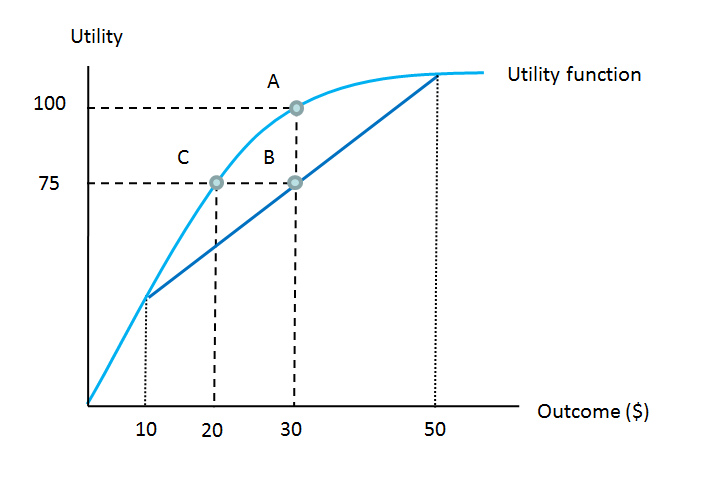
\includegraphics[height=10cm]{img/background/riskaversion}%
    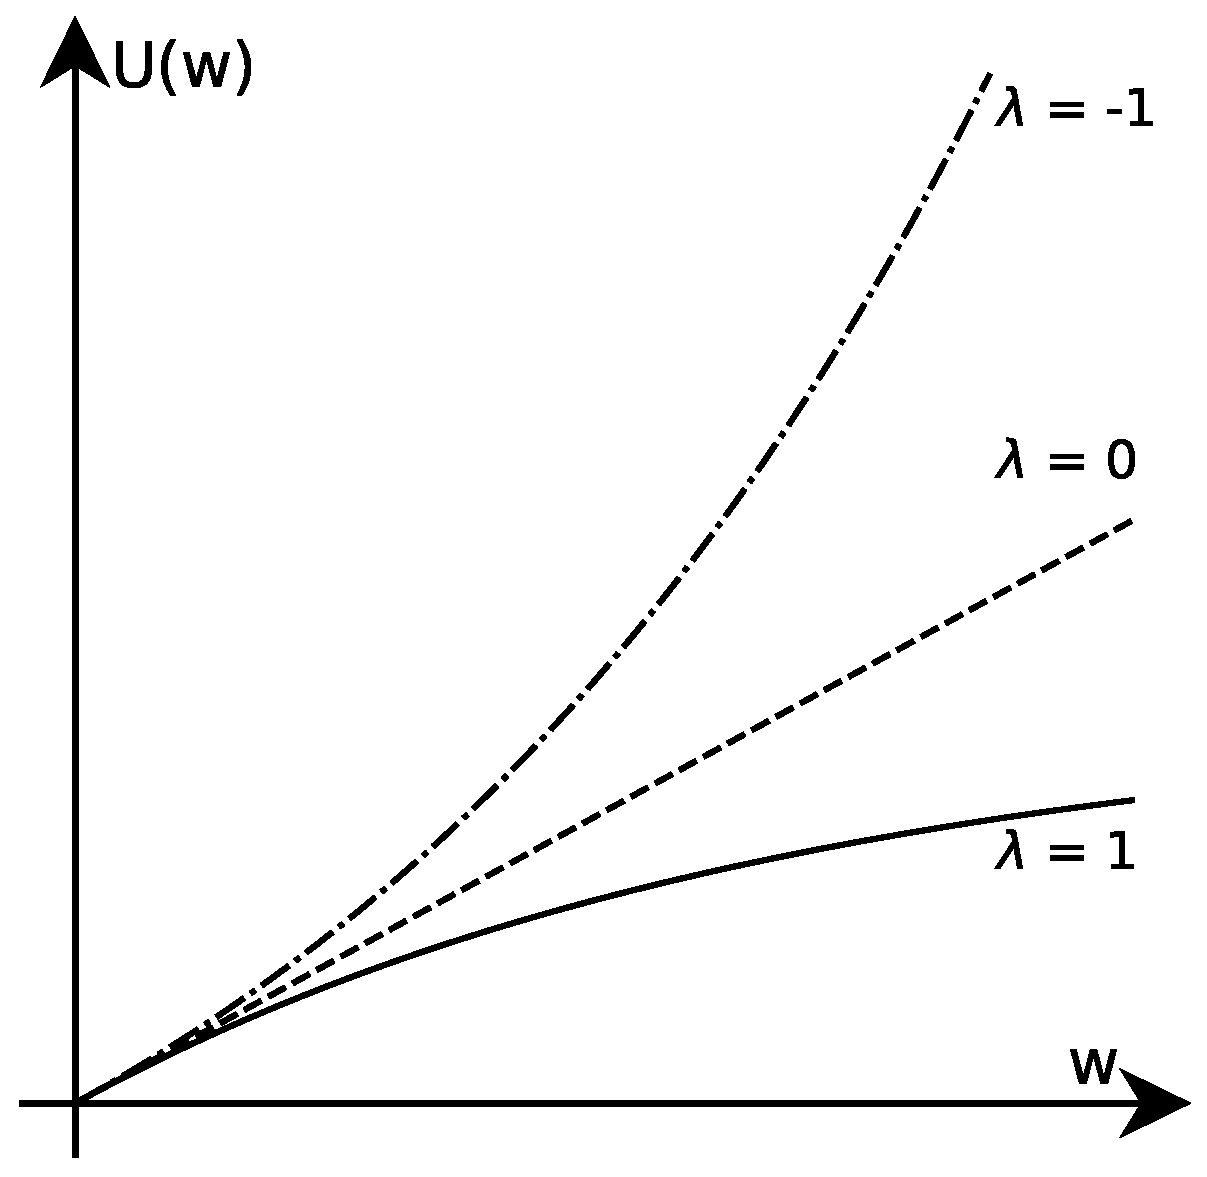
\includegraphics[height=10cm]{img/background/Exponential_Utility_Function}%
  }%
}
\setlength{\twosubht}{\ht\twosubbox}

% typeset

\centering

\subcaptionbox{Risk averse lottery\label{f}}{%
  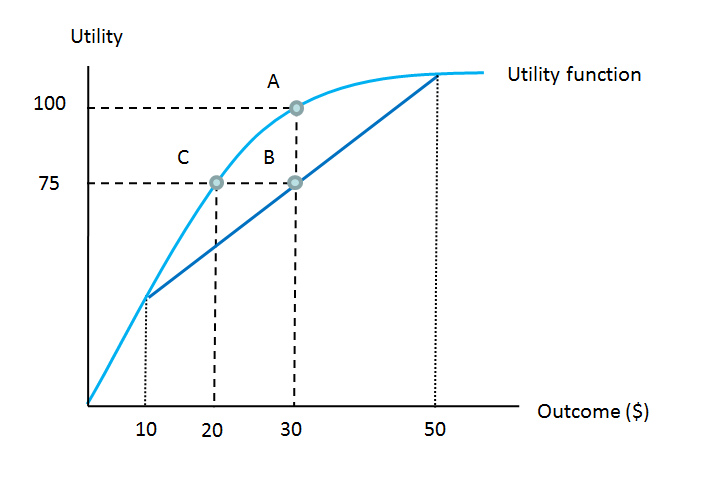
\includegraphics[height=\twosubht]{img/background/riskaversion}%
}\quad
\subcaptionbox{Exponential utility function\label{s}}{%
  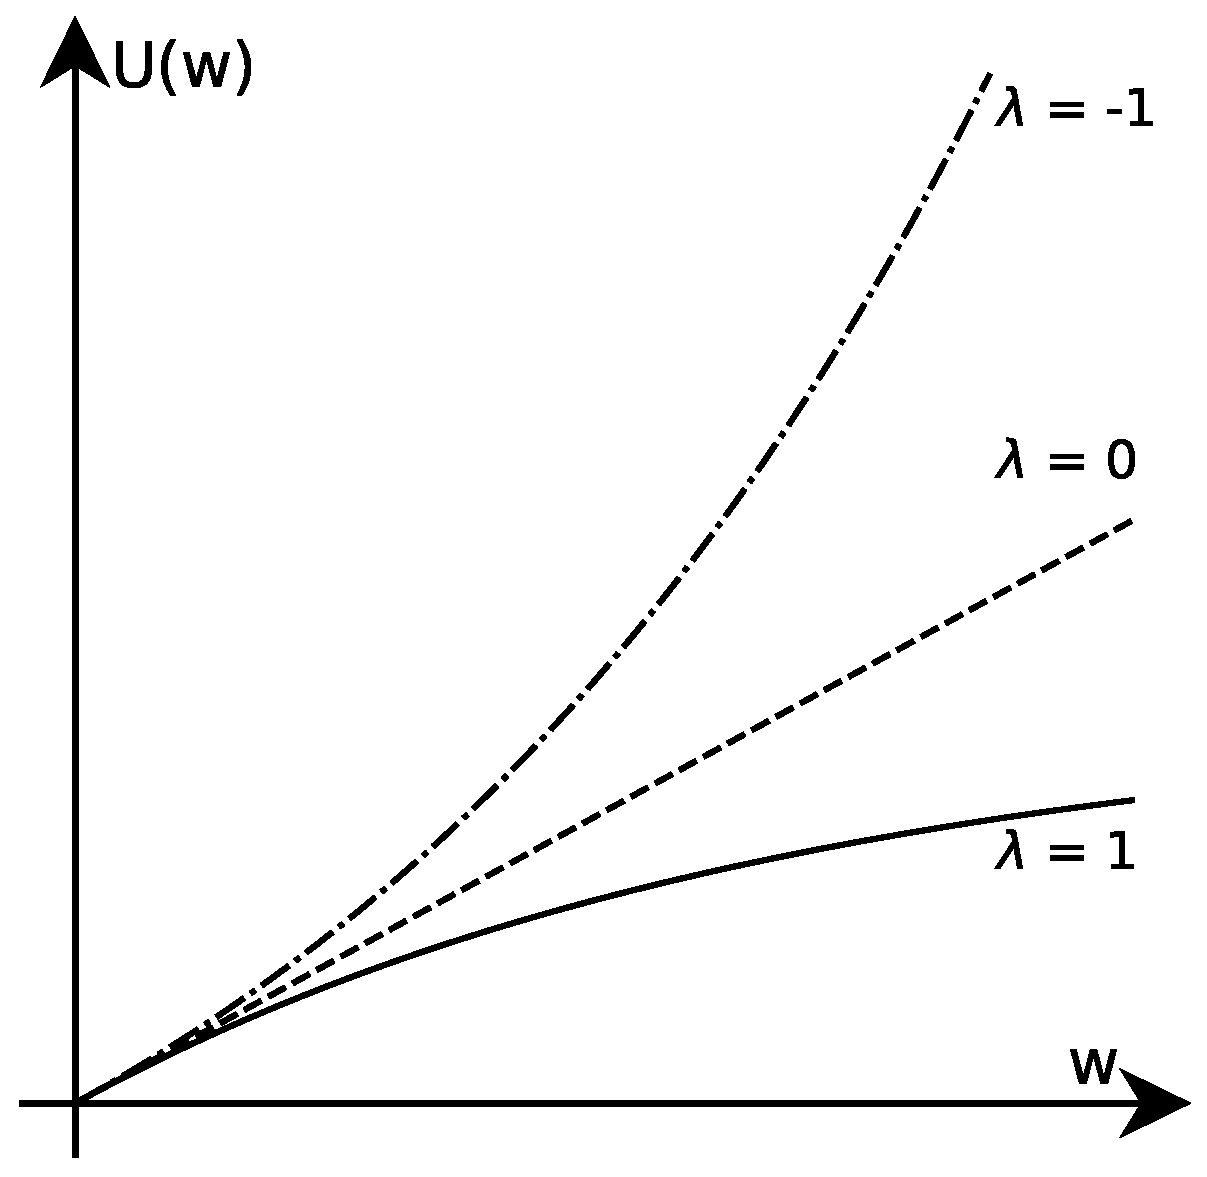
\includegraphics[height=\twosubht]{img/background/Exponential_Utility_Function}%
}

\caption{a) Choice from a risk free gift of 30\$ or a lottery where by coin flip you win 10\$ or 50\$. The utility for the risk free choice (point A) is higher than the expected utility of the risky lottery (point B). b) The exponential utility function for different risk parameters $\alpha$. $a < 0$ implies risk seeking, $a = 0 $ risk neutral and $a > 0 $ risk averse behaviour.}

\end{figure}


\Large{(Partially Observable) Markov Decision Process}

\normalsize
\begin{itemize}
    %\item Making decisions when state is not fully-observable.
    %\item Work on probability distribution over states rather than actual state.
    \item Current state not observable
    \item[$\rightarrow$] Estimate probability of state using observations
\end{itemize}

\hspace{2cm}


\begin{figure}
  \centering
    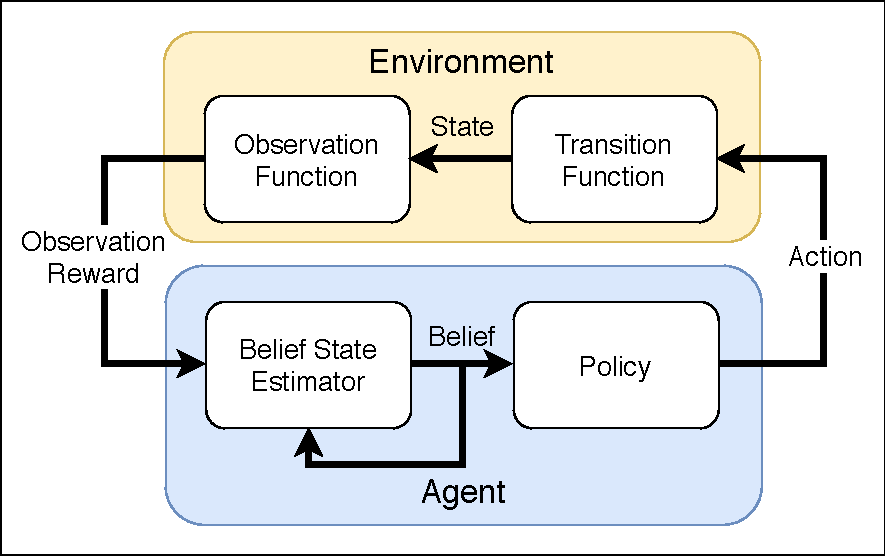
\includegraphics[width=0.7\textwidth]{img/background/POMDP}
  \caption{Sketch of a partially observable environment. The agent only gets observations as inputs.}
\end{figure}


%\begin{itemize}
%    \item Set of States $\mathcal{S}$ (Terminal and Non Terminal)
%    \item Set of Actions $\mathcal{A}$
%    \item Probabilistic Transitions depending on tuple $\mathcal{S} x \mathcal{A}$
%    \item Reward function $R(s,a)$
%\end{itemize}

%For partially observability states are hidden but produce observations:
%\begin{itemize}
%    \item Observation space $\mathcal{O}$
%    \item Observation function $p(o | s, a)$
%\end{itemize}

% add reference: http://www.cassandra.org/arc/papers/aaai94.pdf


\end{exampleblock}



%------------------------------------------------
%----------------------------------------------------------------------------------------

\end{column} % End of the first column

\begin{column}{\sepwid}\end{column} % Empty spacer column

\begin{column}{\onecolwid} % The first column

%----------------------------------------------------------------------------------------
%	OBJECTIVES
%----------------------------------------------------------------------------------------

\begin{exampleblock}{Objectives}

\begin{itemize}
\item Examining behavior of people under risky choice
\item Reassess the assumption that exponential utility function fully explains human risk behavior.
\item Create an artificial agent that behaves in risk-sensitive ways similar to humans, using various utility functions.
\end{itemize}

\end{exampleblock}

%----------------------------------------------------------------------------------------
%	METHODS
%----------------------------------------------------------------------------------------

\begin{exampleblock}{Methods}



\Large{The Experiment}
%TODO Get rid of 4panel, put the top left picture, include text/caption explaining the setting based on picture added
\normalsize
\begin{figure}
\begin {center}
\begin {tikzpicture}[-latex ,auto ,node distance =3cm and 4cm ,on grid ,
semithick ,
state/.style ={ circle ,fill=black!20, minimum width =3 cm}]
\node[state] (C){$Sold$};
\node[state] (A) [above left=of C,align=center] {Reces\\sion};
\node[state] (B) [above right =of C,align=center] {Boom\\ing};
\coordinate[below of=A] (AA);
\coordinate[below of=B] (BB);
\coordinate[below of=AA] (D);
\coordinate[below of=BB] (E);


\path (A) edge [loop left, line width=2mm, align=center] node[left] {wait \\ $0.86$} (A);
\path (A) edge [bend left = -25,line width=2mm,align=center] node[below =0.25 cm] {sell\\$1.0$} (C);
\path (A) edge [bend left =25,line width=2mm,align=center] node[above] {wait\\$0.14$} (B);

\path (B) edge [loop right,line width=2mm,align=center] node[right] {wait\\$1.0$} (B);
\path (B) edge [bend right = -25,line width=2mm,align=center] node[below =0.25 cm] {sell\\$1.0$} (C);

%\fill[gray!40!white, opacity=0.5] (-6,-1) rectangle (5,6);

\path (A) edge [bend right =25,line width=2mm, dashed] node[left] {$Observation$} (D);
\path (B) edge [bend left  =25,line width=2mm, dashed] node[right] {$Observation$} (E);
\end{tikzpicture}
\end{center}
\end{figure}

\begin{itemize}
    \item In a simulated housing market, participants needed to decide whether to sell or to wait.
    \item Waiting decreases risk, but increases costs.
    \item 24 participants performed three different scenarios.
\end{itemize}

\begin{figure}
  \centering
    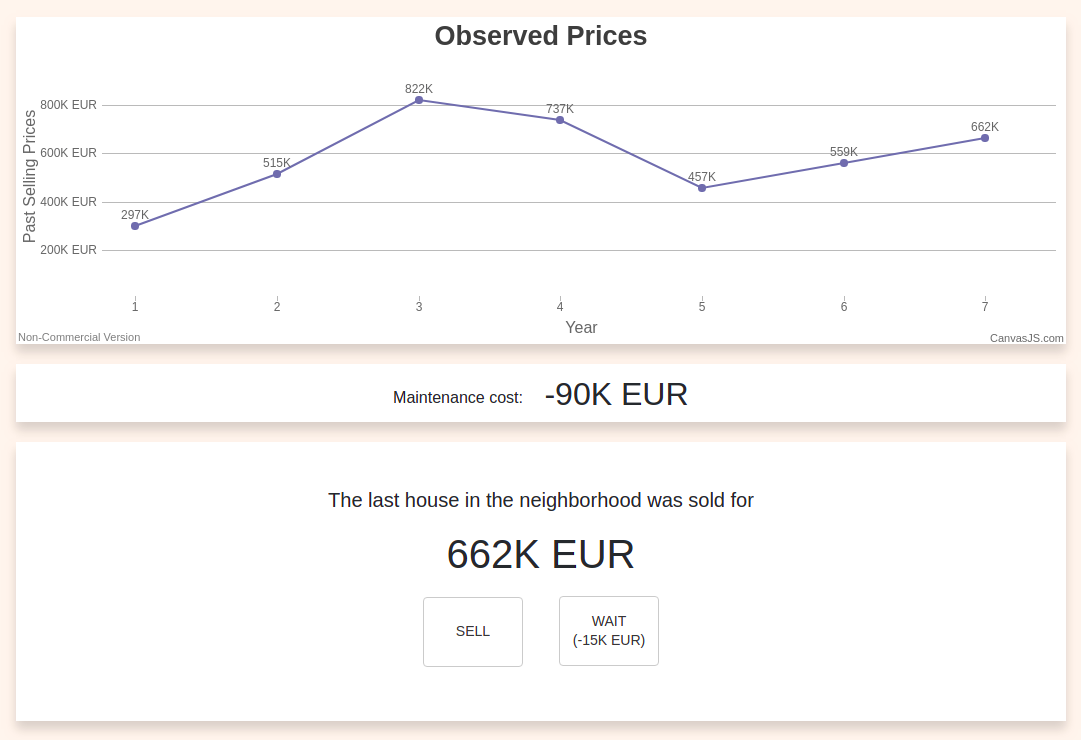
\includegraphics[width=0.8\textwidth]{img/methods/experiment_obs_1.png}
  \caption{Part of the UI used in the experiment showing the observation history.}
\end{figure}


\Large{The Agent}
\normalsize
\begin{itemize}
    \item Simplify POMDP into a MDP by Bayesian estimates.
    \begin{figure}
        \centering
        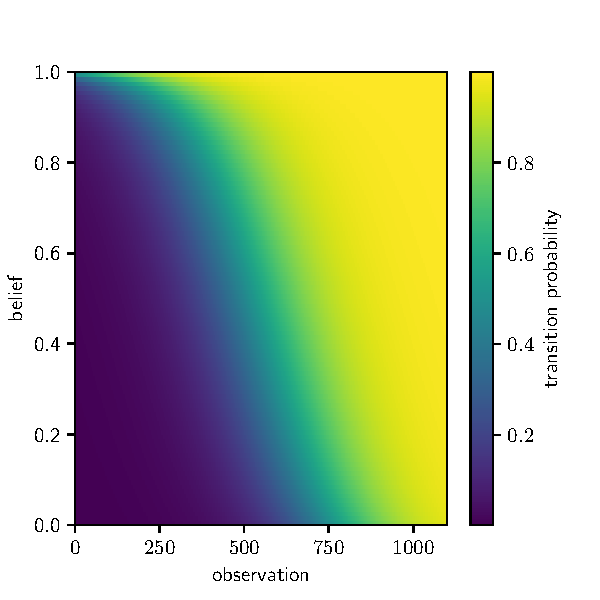
\includegraphics[scale=0.9]{img/belief_table.pdf}
        \caption{Caption}
        \label{fig:my_label}
    \end{figure}
    \item Solve the MDP with value iteration on an augmented state space.
    \begin{flalign}
    V^{n}_{U}(b,w) &= U(w)\tag{Initalization} \\
    V^{n}_{U}(b,w) &= \max_{a \in A}(\sum_{o \in O}{P(o|b)V^{n+1}_{U}(b', w + r(a))}) \tag{Iteration}
    \end{flalign}
    
    \item Different utility functions model different behaviors
    \begin{itemize}
    	\item Time independent (risk parameter $\lambda$)
	 \begin{flalign}
    		U(w)  = \left(1-exp(- \lambda w)\right) / \lambda &&\tag{Exponential utility}
	 \end{flalign}
	 \item Time dependent (risk parameter $\lambda (w)$)
	 \begin{flalign}
    		U(w) &= \left(1-exp(- \lambda(w) w)\right) / \lambda(w)  && \tag{Dynamic Exponential utility}
	 \end{flalign}
	 \item Belief independent (scaling $a$, shift $b$)
	 \begin{flalign}
    		U(w) &= \sinh(a (w-b)) && \tag{Hyperbolic utility}
	 \end{flalign}
	
	 
	
	
	
    \end{itemize}
   
\end{itemize}


\end{exampleblock}

%----------------------------------------------------------------------------------------

\end{column} % End of column 2

%----------------------------------------------------------------------------------------
%	IMPORTANT RESULT
%----------------------------------------------------------------------------------------

%\begin{alertblock}{Important Result}

%Lorem ipsum dolor \textbf{sit amet}, consectetur adipiscing elit. Sed commodo molestie porta. Sed ultrices scelerisque sapien ac commodo. Donec ut volutpat elit.

%\end{alertblock} 

%----------------------------------------------------------------------------------------

\begin{column}{\sepwid}\end{column} % Empty spacer column

\begin{column}{\onecolwid} % The first column within column 2 (column 2.1)

%----------------------------------------------------------------------------------------
%	RESULTS
%----------------------------------------------------------------------------------------
% TODO divide into subsections: Results for Agent, Results for Experiment, Comparison
% TODO make a 3x2 grid with different risks.

\Large{Solving the risk sensitive POMDP}

\normalsize
Marecki \cite{marecki} showed that RSPOMDPs can be solved for arbitrary utility functions using \textbf{reverse value iteration} in Belief Wealth Space.
For this the original state space must be augmented two times:

\begin{figure}
\begin {center}
\begin {tikzpicture}[-latex ,auto ,node distance =8cm and 6cm ,on grid ,
semithick ,
state/.style ={ circle ,fill=black!20, minimum width =6 cm}]
\node[state] (A) [align=center] {Observation\\Time\\Space};
\node[state] (B) [right of=A,align=center] {Belief\\Time\\Space};
\node[state] (C) [right of=B,align=center] {Belief\\Wealth\\Space};


\path (A) edge [line width=2mm, align=center] node[left] {} (B);
\path (B) edge [line width=2mm,align=center] node[below =0.25 cm] {} (C);
\end{tikzpicture}
\end{center}
\end{figure}

\hspace{2cm}

\Large{Value functions in belief wealth space}


\normalsize

\begin{figure}
    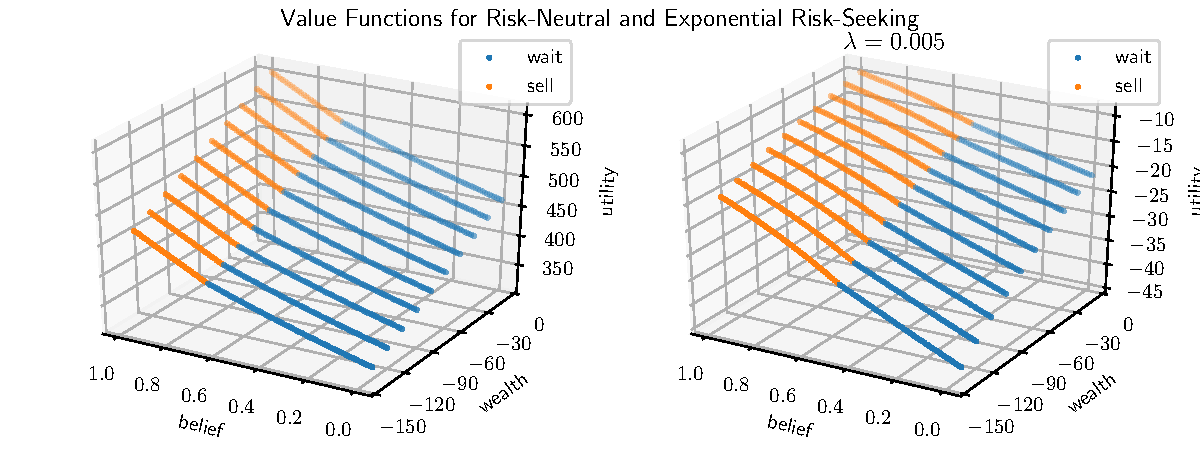
\includegraphics[width=0.98\linewidth]{img/exp_policy.pdf}\\
    \vspace{1cm}
    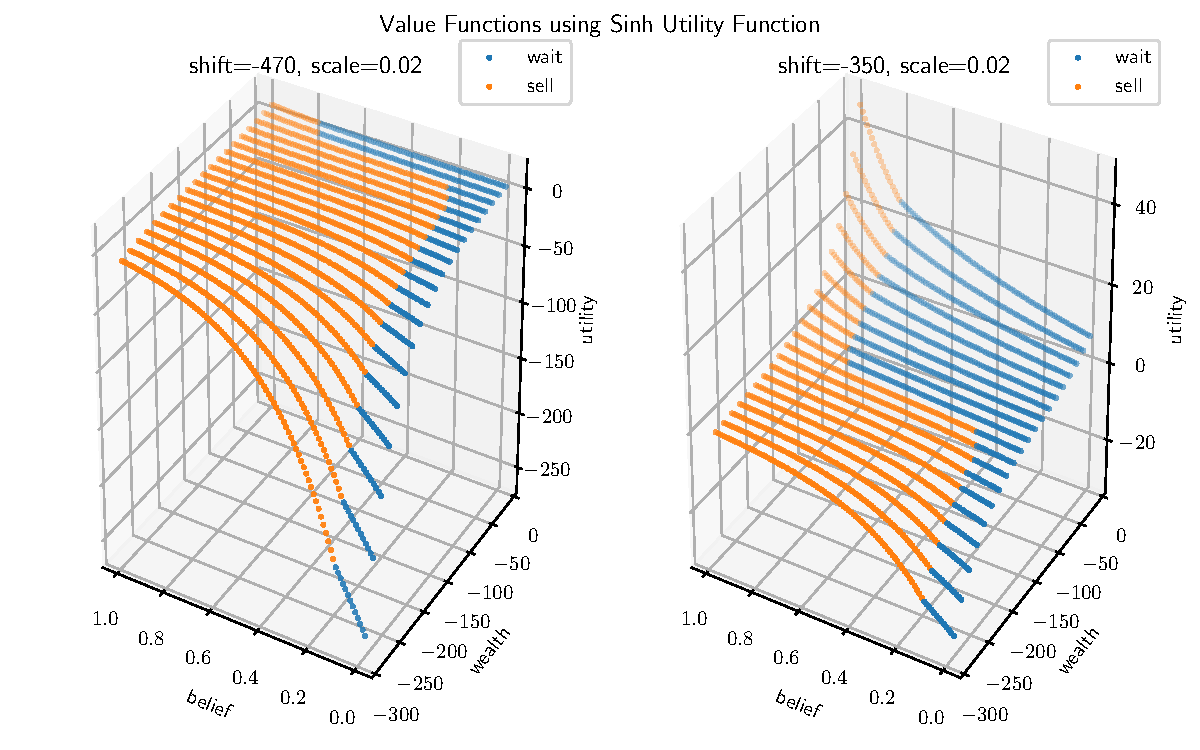
\includegraphics[width=0.98\linewidth]{img/sinh_policy.pdf}\\
    \vspace{1cm}
    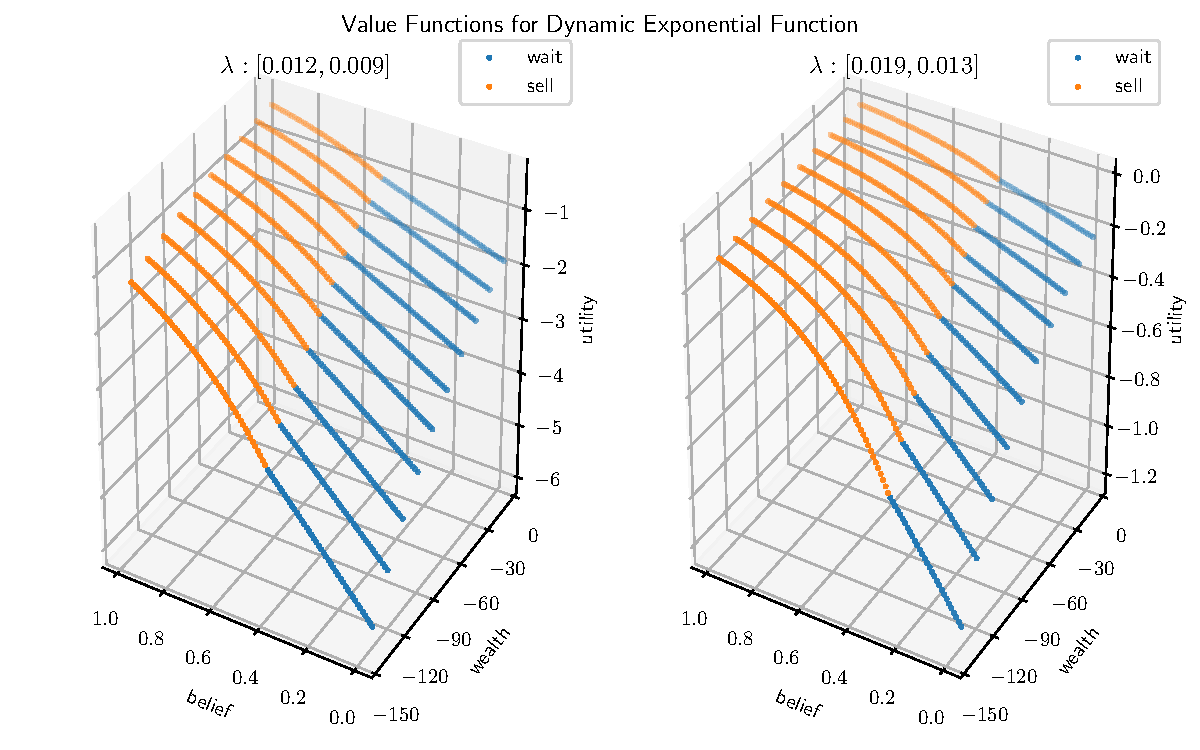
\includegraphics[width=0.98\linewidth]{img/dyn_policy.pdf}
    \caption{Value functions exhibiting different risk-behaviors; from top left: risk neutral agent (utility function is the identity function), risk-seeking agent with exponential utility function, two fixed time agents with different time thresholds, two agents with dynamic exponential utility function.}
\end{figure}

\Large{From human behavior to utility functions}


\normalsize
\textbf{The original problem:}
\begin{itemize}
\item[①] Choose utility function with risk parameter.
\item[②] Perform value iteration.
\item[③] Derive policy.
\end{itemize}

\textbf{The inverse problem:}
\begin{itemize}
\item[①] Observe behavior.
\item[②] Estimate policy.
\item[③] Derive utility function and risk parameters.
\end{itemize}

The original problem is easy to solve, unfortunately for the inverse problem no solution is known. 

$\rightarrow$ Perform grid-search and choose optimal utility function.


%\begin{table}
%\vspace{2ex}
%\begin{tabular}{l l l}
%\toprule
%\textbf{Treatments} & \textbf{Response 1} & \textbf{Response 2}\\
%\midrule
%Treatment 1 & 0.0003262 & 0.562 \\
%Treatment 2 & 0.0015681 & 0.910 \\
%Treatment 3 & 0.0009271 & 0.296 \\
%\bottomrule
%\end{tabular}
%\caption{Table caption}
%\end{table}

\end{exampleblock}

%----------------------------------------------------------------------------------------

\end{column} % End of the third column

\begin{column}{\sepwid}\end{column} % Empty spacer column

\begin{column}{\onecolwid} % The third column

%----------------------------------------------------------------------------------------
%	DISCUSSION
%----------------------------------------------------------------------------------------

\begin{exampleblock}{Discussion}

\begin{itemize}
    \item 
\end{itemize}

\end{exampleblock}

%----------------------------------------------------------------------------------------
%	ADDITIONAL INFORMATION
%----------------------------------------------------------------------------------------

\begin{exampleblock}{Additional Information}

Maecenas ultricies feugiat velit non mattis. Fusce tempus arcu id ligula varius dictum. 
\begin{itemize}
\item Curabitur pellentesque dignissim
\item Eu facilisis est tempus quis
\item Duis porta consequat lorem
\end{itemize}

\end{exampleblock}

%----------------------------------------------------------------------------------------
%	REFERENCES
%----------------------------------------------------------------------------------------

\begin{exampleblock}{References}

\nocite{*} % Insert publications even if they are not cited in the poster
\small{\bibliographystyle{unsrt}
\bibliography{sample}\vspace{1cm}}
\end{exampleblock}

%----------------------------------------------------------------------------------------
%	ACKNOWLEDGEMENTS
%----------------------------------------------------------------------------------------

%\setbeamercolor{block title}{fg=red,bg=white} % Change the block title color

%\begin{exampleblock}{Acknowledgements}

%\small{\rmfamily{Nam mollis tristique neque eu luctus. Suspendisse rutrum congue nisi sed convallis. Aenean id neque dolor. Pellentesque habitant morbi tristique senectus et netus et malesuada fames ac turpis egestas.}} \\

%\end{exampleblock}

%----------------------------------------------------------------------------------------
%	CONTACT INFORMATION
%----------------------------------------------------------------------------------------

%\setbeamercolor{block alerted title}{fg=black,bg=norange} % Change the alert block title colors
%\setbeamercolor{block alerted body}{fg=black,bg=white} % Change the alert block body colors

\begin{block}{Contact Information}

\begin{itemize}
\item Web: \href{http://ideal1st.com/}{http://ideal1st.com/}
\item Email: \href{mailto:ideal1st.here@gmail.com}{ideal1st.here@gmail.com}
\end{itemize}

\end{block}

\begin{block}{Acknowledgements}

This work was supported by [Department Name]. The authors gratefully acknowledge the helpful discussions and technical assistance provided by [Rong], [Vaios].
We also thank the WZB department for assisting us during the execution of the experiment.

\end{block}

%----------------------------------------------------------------------------------------

\end{column} % End of the third column

\begin{column}{\sepwid}\end{column} % Empty spacer column

\end{columns} % End of all the columns in the poster

\end{frame} % End of the enclosing frame
%\end{darkframes} % Uncomment for dark theme
\end{document}
